Effortlessly communicating with computers using natural language has
been a longstanding goal of artificial intelligence~\cite{Winograd71}.
Reinforcement Learning (RL) presents a flexible framework for
optimizing goal oriented behavior~\cite{sutton18}. As such, one can
use RL to optimize language communication if it is expressed in terms
of achieving concrete goals.  In this pursuit, researchers have
created a number of simulation environments where a learning agent is
provided with a natural language input and asked to produce a sequence
of actions for achieving a goal specified in the input
text~(\eg~\citet{long16,hermann17,chaplot18,fu19,babyai}).  These
tasks are typically episodic, where the agent receives sparse binary
success-failure feedback indicating whether an intended goal has been
accomplished.  After training, the agent is placed in new contexts and
evaluated based on its ability to reach novel goals, indicating the quality
of its behavior policy and language interpretation skills. The
emphasis on generalization in these tasks makes them
suitable for benchmarking overfitting in
RL~\cite{cobbe2018quantifying, zhang2018study}.

\begin{figure}[t]
\small
\begin{tabular}{@{}l@{\hspace*{.3cm}}l@{}}
\begin{tabular}{@{}|@{\ww}l@{\ww}l@{\ww}l@{\ww}l@{\ww}|@{}}
\hline
Rank & Nation & Gold & Silver \\%& Bronze & Total\\
\hline
1 & USA	&	10 &	12 \\%&	9 \\%&	35 \\
2 & GBR	&	9 &	4 \\%&	4 \\%&	17 \\
3 & CHN	&	8 &	11 \\%&	4 \\%&	23 \\
4 & RUS &	2 &	4 \\%&	7 \\%&	13 \\
5 & GER &	2 &	2 \\%&	2 \\%&	6 \\
6 & JPN & 	2 &	1 \\%&	3 \\%&	6 \\
7 & FRA &	2 &	1 \\%&	0 \\%&	3 \\
\hline
%\bottomrule
\end{tabular}%
&
\raisebox{1.2cm}{\begin{minipage}[t]{4.65cm}
$\vx$ = ``Which nation won the most\\silver medal?''\\
$R(\va) = \one{\texttt{Execute}(\va) = \text{``USA''}}$\\[.3cm]
$\va_1$ = \texttt{argmax\_row(}Silver\texttt{)}.Nation\\
$\va_2$ = \texttt{argmax\_row(}Gold\texttt{)}.Nation\\
$\va_3$ = \texttt{argmin\_row(}Rank\texttt{)}.Nation\\
$R(\va_1) = R(\va_2) = R(\va_3) = 1$
\vfill
\end{minipage}}
\\
\end{tabular}

\caption{{\em Semantic parsing} from question-answer pairs. An agent is presented with a natural language question $\vx$
and is asked to generate a SQL-like program $\va$. The agent receives
a reward of $1$ if execution of a program $\va$ on the relevant data
table leads to the correct answer (\eg~USA).  The reward is
underspecified because {\em spurious} programs (\eg~$\va_2, \va_3$) can
also achieve a reward of $1$. }
\label{fig:fig1}
\end{figure}

\begin{figure}[t]
\small
\begin{tabular}{@{}l@{\hspace*{.1cm}}l@{}}
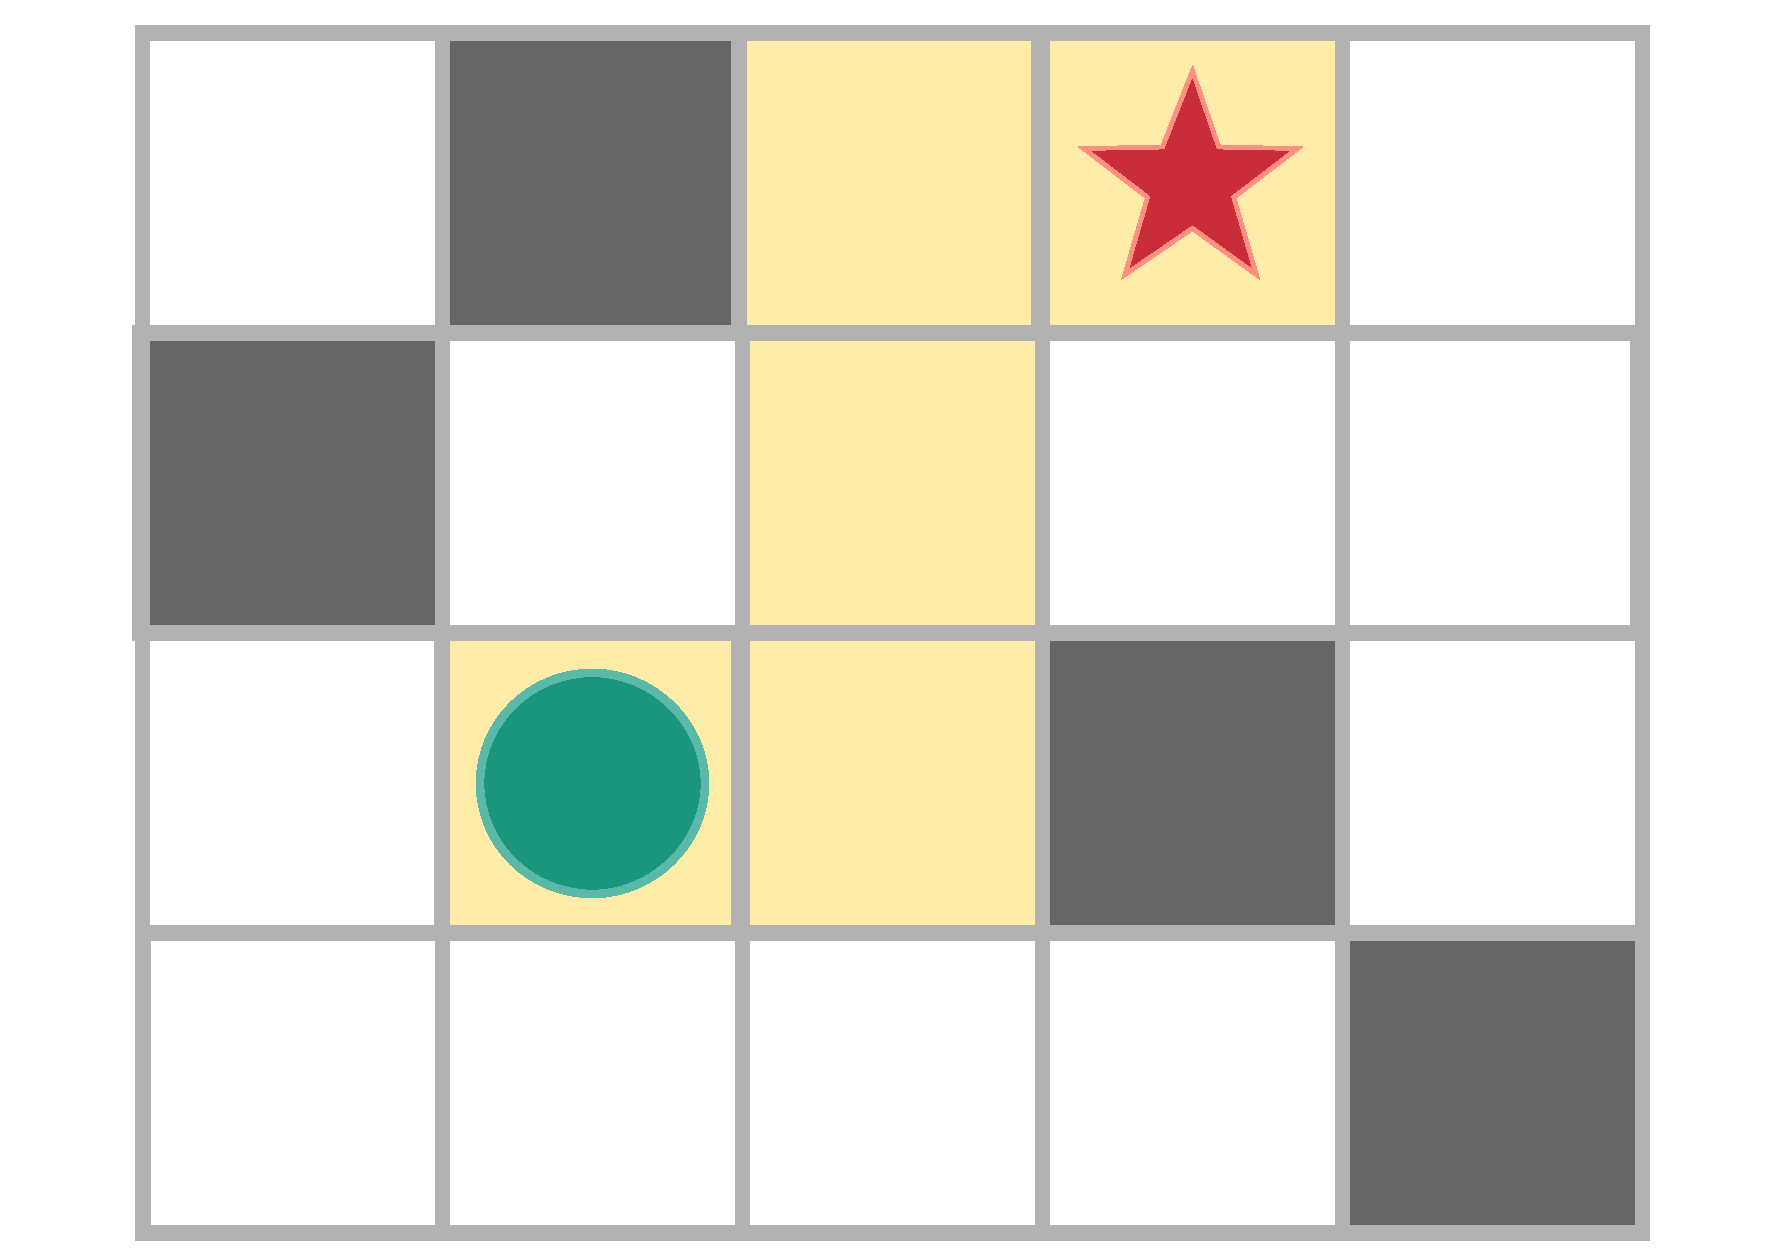
\includegraphics[width=3.4cm]{diagram.pdf}
&
\raisebox{2.15cm}{\begin{minipage}[t]{4.3cm}
$\vx$ = ``Right Up Up Right''\\
$R(\va) = \one{\texttt{Execute}(\bullet,\va) = \star}$\\[.3cm]
$\va_1 = (\rightarrow, \uparrow, \uparrow, \rightarrow)$\\
$\va_2 = (\leftarrow, \rightarrow, \rightarrow, \uparrow, \uparrow, \rightarrow)$\\
$\va_3 = (\uparrow, \rightarrow, \rightarrow, \uparrow)$\\
$R(\va_1) = R(\va_2) = R(\va_3) = 1$
\vfill
\end{minipage}}
\\
\end{tabular}

\caption{{\em Instruction following} in a simple maze. A blind agent is presented with
a sequence of (Left, Right, Up, Down) instructions. Given the input
text, the agent ($\bullet$) performs a sequence of actions, and only
receives a reward of $1$ if it reaches the goal ($\star$).}
\label{fig:fig2}
\vspace*{-0.15in}
\end{figure}

\figref{fig:fig1} and \ref{fig:fig2} illustrate two examples
of contextual environments with sparse and underspecified rewards.
The rewards are {\em sparse}, since only a few trajectories in the
combinatorial space of all trajectories leads to a non-zero return.
In addition, the rewards are {\em underspecified}, since the agent may
receive a return of $1$ for exploiting {\em spurious} patterns in the
environment.  We assert that the generalization performance of an
agent trained in this setting hinges on (1) effective exploration to
find successful trajectories, and (2) discounting spurious
trajectories to learn a generalizable behavior.

To facilitate effective and principled exploration,
we propose to disentangle combinatorial search and exploration
from robust policy optimization. In particular, we use a {\em mode
covering} direction of KL divergence to learn a high entropy
exploration policy to help collect a diverse set of successful
trajectories.
Then, given a buffer of promising trajectories,
we use a {\em mode seeking} direction of KL divergence
to learn a robust policy
with favorable generalization performance.

A key challenge in language conditional learning environments is the
lack of fully specified rewards that perfectly distinguish optimal
and suboptimal trajectories.  Designing a rich trajectory-level
reward function requires a deep understanding of the semantic
relationship between the environment and the natural language input,
which is not available in most real-world settings.  Such a challenge
arises in weakly supervised semantic parsing as depicted
in \figref{fig:fig1}~\cite{pasupat2015tables}.  From an AI safety
perspective, underspecified rewards may lead to reward
hacking~\cite{amodei2016concrete} causing unintended and harmful
behavior when deployed in real-world scenarios.

In this paper, we investigate whether one can automatically discover a
rich trajectory-level reward function to help a learning agent
discount spurious trajectories and improve generalization.  Toward
this end, we utilize both gradient-based
Meta-Learning~\cite{finn2017model,maclaurin2015gradient} and Bayesian
Optimization~\cite{snoek2012practical} for reward learning. We propose
to optimize the parameters of the auxiliary reward function in an
outer loop to maximize generalization performance of a policy trained
based on the auxiliary rewards. Our work is distinct from recent
works~\cite{bahdanau19, fu19} on learning rewards for language tasks because
we do not require any form of trajectory or goal demonstration.

We evaluate our overall approach (see Figure \ref{fig:fig3} for an
overview) on two real world weakly-supervised semantic parsing
benchmarks~\cite{pasupat2015tables,zhong2017seq2sql}
(\figref{fig:fig1}) and a simple instruction following environment
(\figref{fig:fig2}).  In all of the experiments, we observe a
significant benefit from the proposed Meta Reward Learning~(MeRL)
approach, even when the exploration problem is synthetically
mitigated.  In addition, we achieve notable gains from the mode
covering exploration strategy, which combines well with MeRL to
achieve the state-of-the-art results on weakly-supervised semantic
parsing.

\begin{figure}[t]
\begin{center}
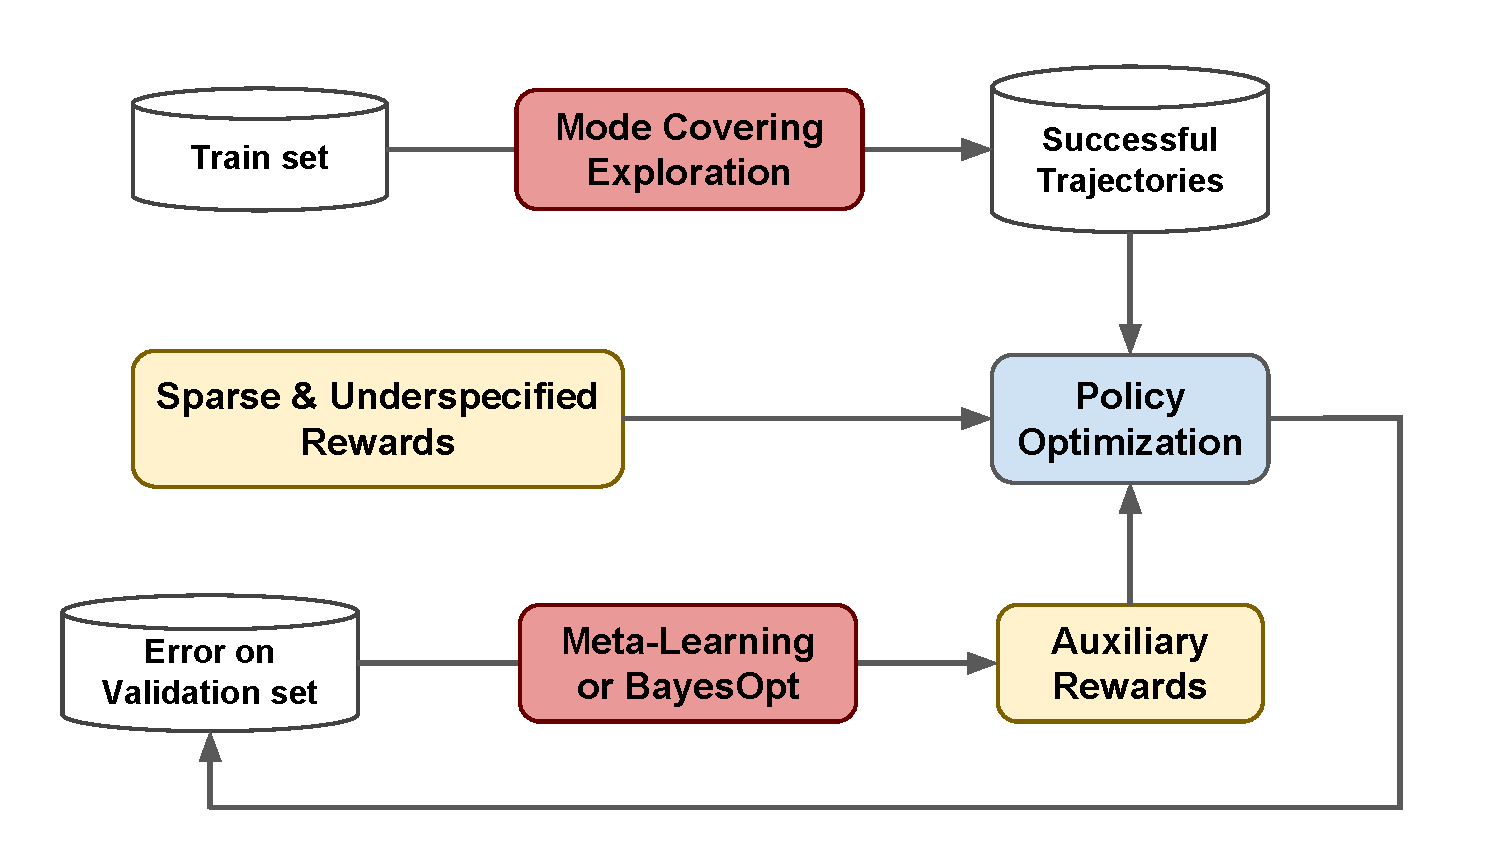
\includegraphics[width=1.0\columnwidth]{fig_method.pdf}
\end{center}
\vspace{-.15in}
\caption{Overview of the proposed approach. We employ (1) mode covering exploration to collect a diverse set of successful trajectories in a memory buffer;
(2) Meta-learning or Bayesian optimization to learn an auxiliary reward function to discount spurious trajectories.}
\label{fig:fig3}
\vspace{-.05in}
\end{figure}
